\section{Measure Theoretic Approach}

Assume a discrete time setup $t\in\N$.
Suppose at time $t = 0$ we have a population consisitng of $i\in\left\{ 1, 2, \ldots, I \right\}$ individuals,
each of age $a_i\in\N$. Suppose offspring production is a random process,
iid between individuals, determined by age $a$; that is, $X(a)$ is the random variable specifying the number of offspring produced, or $-1$ if 
the individual dies. Then the population the following time step is 
$$ \text{pop}(1) = I + \sum\limits_{i = 1}^I X_i(a_i).$$
More poignantly, the \textit{relative} population size is:
$$\frac{1}{I}\text{pop}(1) = 1 + \frac{1}{I}\sum\limits_{i = 1}^I X_i(a_i)$$
Perhaps even \textit{MORE} poignantly, the relative population size in expectation is:
\begin{align*}
    E\left[\frac{1}{I}\text{pop}(1)\right] &= 1 + \frac{1}{I}\sum\limits_{i = 1}^I g(a_i) \\
    &= 1 + \int_0^\infty g(a) d\mu(a)
\end{align*}
where $g$ is the offspring minus death mass function and $\mu$ is the distribution on
$\N$ specifying the proportion of the population in each age class $a\in\N$. We generalize immediately,
and claim that in discrete time, fitness is defined by:
$$ r = 1 + \sum\limits_0^\infty g(a) \mu(a) = 1 + \int_0^\infty g(a) d\mu(a), $$
where once more $g$ is the birth density function minus the death density function, and $\mu$ is a probability
measure on $\R_{> 0}$ specifying the distribution of the population. Generalizing even further, the population growth rate
is just
$$ \int_0^\infty g(a) d\mu(a) $$
which applies equally to continuous and discrete time models. So are we done? Of course not! Look at how much is left to be read on
the next page! Continue with discrete time as our motivating set up; everything will (hopefully) translate well enough to continuous
time. We began with a distribution $\mu$ providing the fraction of the population in each age category; call it $\mu_0 = \mu$. After
everybody gives birth and gets older, we have a new age distribution, $\mu_1$. Concretely,
$$ \mu_1(a) = 
\begin{cases}
    \sum\limits_0^\infty g(a) \mu_0(a) & \text{ if  } a = 0 \\
    (1 - \delta(a-1))\mu_0(a-1) & \text{ else.}
\end{cases}
$$
In the above, $\delta(\cdot)$ is the function specifyiing the probability of dying at age $a$, so that $1-\delta$ is survival probability.
To make $\mu_1$ a probability measure, we need to rescale so that $\mu_1(\R) = 1$; set $\mu_1 = \frac{1}{r_1}\mu_1$. We can similarly define
$\mu_t$ recursively for each $t\in\N$. A natural question is: does our age distribution stabalize down to something nice? That is, does
$\mu_t(a)\to \nu(a)$ for each $a\in\N$? 

\subsection{For concreteness, Leslie matrices as an example}
Everything above was highly abstract; how am I so convinced that what I've written is correct? Fortunately, the Leslie model 
encorporates all of the elements above, and so allows us to check: does this all okay? Suppose we have three age classes,
$a\in\left\{ 0, 1, 2 \right\}$, survival probabilities $s_0, s_1, s_2 = 0$, and birth rates $b_0, b_1, b_2$. This setup produces the
standard Leslie matrix:
$$ L = 
\begin{pmatrix}
    b_0 & b_1 & b_2 \\
    s_0 & 0 & 0 \\
    0 & s_1 & 0 \\
\end{pmatrix}
$$
Translating to the setup above, we have $g(a) = b_a - s_a$. As per standard Leslie model stuff, we have a stable age distribution:
call it $(n_0, n_1, n_2)$. By setting $\mu(a) = n_a$, we can experimentally check: does
$$ \sum g(a)\mu(a) = r$$
where $r$ is the leading eigenvalue of $L$? I checked and it worked once, so I figure yes, it must hold in general. 

\subsection{Back to abstract measure theory stuff}
What we are looking at very closely resembles a Markov chain. I'm hopeful that we can co-opt the tools from Markov Chain Theory to
prove that under analogous conditions to aperiodicity, there exists a unique stationary measure $\mu$ for our population growth
process to which the $\mu_t$ converge (what exactly is meant by convergence is to be determined).  
\subsection{Corrections}

Last week, I told some lies, which I will now try to rectify. On the one hand, if $\beta, \delta$ are instantaneous birth and
death rates as a function of age (assuming we have reached a given age), then we do indeed have:
$$ r = \int_0^\infty (\beta(a) - \delta(a))d\mu(a) = \int_0^\infty(\beta(a) - \delta(a))n(a) da. $$
We can get away from using a measure $\mu$ to multiplying by the stable age distribution due to Radon-Nikodym. The picture I tried
to use to motivate all of this work is slightly different. The graph showing the ``typical life history'' of a squirrel actually corresponds
to the function $\beta(a)\cdot s(a)$, where $\beta$ is as above and $s$ is the probability of surviving to age $a$. Then the question is:
for what measure $\Delta$ does 
$$ \int_0^\infty \beta(a) s(a) d \Delta(a)?$$
We use $\Delta$ for discounting, since $\delta$ is already used for the instantaneous death rate. By a simple re-arrangement, we can write
\begin{align*}
    r &= \int (\beta(a) - \delta(a))n(a) da \\
    &= \int \beta(a) s(a) \frac{\beta(a) - \delta(a)}{\beta(a) s(a)} n(a) d a.
\end{align*}
So interestingly, we can take
$$ \Delta(a) = \frac{\beta(a) - \delta(a)}{\beta(a) s(a)} n(a).  $$
``Why is this interesting?'' you might ask. Well, for one thing $\Delta(a) < 0$ whenever $\beta < \delta$. Further, $\Delta$ need not be
decreasing. Nevertheless, this is something to work with.



\subsection{Examples of life history displays}
For the sake of concreteness, as well as tying squirrel banking together with this abstract nonsense, we can compute
the expected life history of a squirrel saving to different $\hat \beta$. In particular, for $(p_0, p_1, p_2) \approx
(0.1089, 0.4725, 0.4186)$, we have the following life histories:

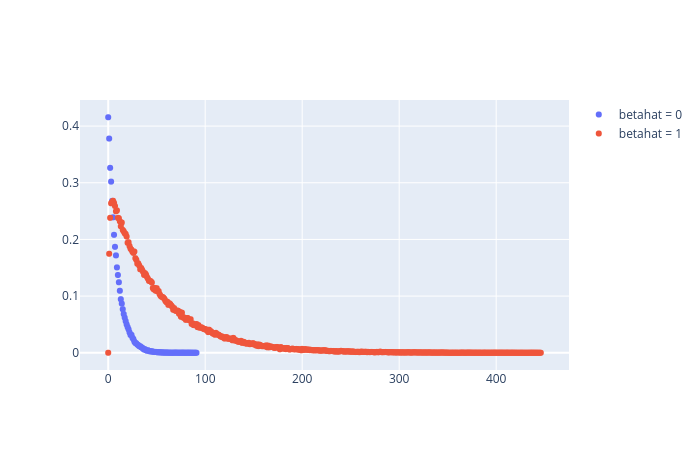
\includegraphics[scale = 0.8]{life_histories} \\

We chose these values for $p_0,p_1, p_2$ because at this distribution of nuts, the fitness for $\hat \beta = 0$ is about the same
as that of $\hat \beta = 1$. 
Each point represents the expected number of offspring a squirrel produces on a given day in its life, with the horizontal axis being
time. Below, it is more zoomed in.

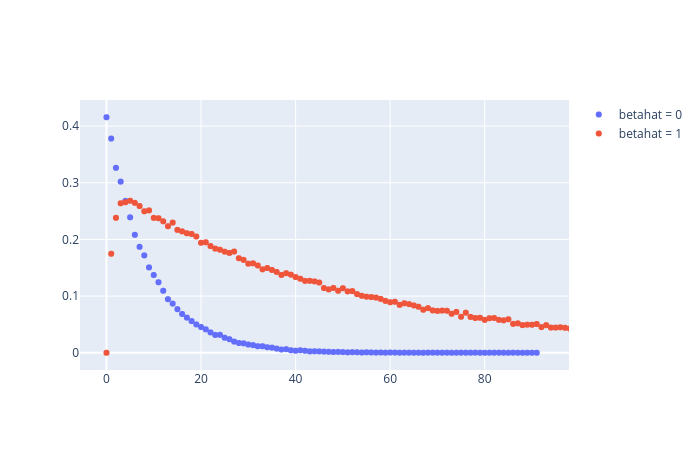
\includegraphics[scale = 0.8]{zoomed_life_histories} \\

\subsection{Summing up all contributions}
I am still pathologically trying to get life history to tell a discounting story. In particular, I want to find a 
discounting function $\Delta(a,q)$ satisfying
$$ \int_0^\infty \beta(a) s(a) \Delta(a, \beta(a) s(a)) d a = \text{ fitness.} $$
In what follows, $q$ can be thought of as ``quantity of offspring produced.'' For any measure of fitness, we have
$$ \text{fitness } = \text{ fitness}(q_{1}, q_{2}, \ldots ),$$
with $q_a$ the quantity of offspring at age $a$. Let's assume (and this is a significant assumption) that we can decompose the different
contributions to fitness as 
$$ \text{fitness } = \sum\limits_{a = 1}^\infty C(a, q_a),$$
with $C(a, q_a)$ representing the total contribution to fitness of quantity $q_a$ at age $a$. This is a significant assumption since it
implies that
$$ \frac{\partial}{\partial q_{a}} \text{fitness } = \frac{\partial}{\partial q_{a}} C(a, q_a). $$
In particular, varying the quantity you produce on a given day does not impact the contribution to fitness on other days. This seems sort of
unreasonable, but we proceed nevertheless. By the fundamental theorem of calculus, we know that
$$ C(a, q_a) = \int_0^{q_a} \frac{\partial}{\partial q} C(a, q) d q = q_a \mathbb{E}_0^{q_a}\left[ \text{MCF}_a \right]. $$
In the above, $\text{MCF}_a$ is the marginal contribution to fitness. Plugging this into our expression for fitness, we have
$$ \text{fitness } = \sum\limits_{a = 1}^\infty q_a \mathbb{E}_0^{q_a}\left[ \text{MCF}_a \right].$$ 
Thus taking $\Delta(a, q_a) = \mathbb{E}_0^{q_a}\left[ \text{MCF}_a \right]$ produces a discounting function which gives back
fitness. \\\\

\textbf{Pure Leslie Matrix analysis} \\\\

Assume a Leslie model setup: we have a maximal age of $A \le \infty$, day to day survival probability is $s_1, s_2, \ldots, s_{A-1}$,
and fecundity is $b_1, b_2, \ldots, b_A$. The Euler-Lotka equation is:

$$ \lambda^A = \sum\limits_{a = 1}^A \lambda^{A-a}s_1 s_2 \cdots s_{a-1} b_a.$$

We can use implicit differentiation (or the semi-valid $\frac{\d \lambda}{ \d b_\alpha} = \frac{\d EL}{\d b_\alpha}/
\frac{\d EL}{\d \lambda}$) to obtain:

\begin{align*}
    \frac{\d \lambda}{\d b_{\alpha}} &= \frac{\lambda^{A-\alpha}s_1s_2\cdots s_{\alpha-1}}{A\lambda^{A-1} -
    \sum\limits_{a = 1}^{A-1}s_1s_2\cdots s_{a-1}b_a\lambda^{A-a-1}} \\\\
    &= \frac{\lambda^{A-\alpha}}{\lambda^{A-1}} \cdot \frac{s_1s_2\cdots s_{\alpha-1}}{A - \sum\limits_{a = 1}^{A-1}s_1s_2\cdots s_{a-1}b_a\lambda^{-a}}\\\\
    &= \lambda^{1-\alpha} \cdot \frac{s_1s_2\cdots s_{\alpha-1}}{A - \sum\limits_{a = 1}^{A-1}s_1s_2\cdots s_{a-1}b_a\lambda^{-a}},
\end{align*}
where $\alpha\in\left\{ 1, 2, \ldots, A \right\}$ is arbitrary. This seems to be getting us nowhere! Nevertheless, we continue by
noting that $\frac{\d \lambda}{\d b_\alpha} = \text{MCF}_\alpha$, so that our proposed discounting function above turns out to be:

\begin{align*}
    \Delta(\alpha, q(b_\alpha)) &=\frac{1}{q(b_{\alpha})} \mathbb{E}_0^{q(b_\alpha)}\left[ \text{MCF}_\alpha\right] \\
    &= \frac{1}{q(b_{\alpha})} \int_0^{q(b_\alpha)} \lambda^{1-\alpha} \cdot \frac{s_1s_2\cdots s_{\alpha-1}}{A - \sum\limits_{a = 1}^{A-1}s_1s_2\cdots s_{a-1}b_a\lambda^{-a}} \d b_\alpha \\
    &= \frac{\lambda^{1-\alpha}}{s_1s_2\cdots s_{\alpha-1}b_{\alpha}}\cdot\int_0^{q(b_\alpha)} \frac{s_1s_2\cdots s_{\alpha-1}}{A - \sum\limits_{a = 1}^{A-1}s_1s_2\cdots s_{a-1}b_a\lambda^{-a}} \d b_\alpha \\
    &= \frac{\lambda^{1-\alpha}}{b_{\alpha}}\cdot\int_0^{q(b_\alpha)} \frac{1}{A - \sum\limits_{a = 1}^{A-1}s_1s_2\cdots s_{a-1}b_a\lambda^{-a}} \d b_\alpha \\
\end{align*}

This is starting to look like something more interesting - of particular note is the fact that we have an exponential discounting term $\lambda^{1-\alpha}$
floating around in there. For sufficiently large $b_{\alpha}$, notice that $\lambda\to\infty$ so that $\lambda^{-a}\to 0$ for each 
$a\in\left\{ 1, 2, \ldots, A-1 \right\}$. Thus, for $b_\alpha$ sufficiently large, the integrand begins to look like

\begin{align*}
    \int_0^{q(b_\alpha)} \frac{1}{A - \sum\limits_{a = 1}^{A-1}s_1s_2\cdots s_{a-1}b_a\lambda^{-a}} \d b_\alpha &\to  \int_0^{q(b_\alpha)} \frac{1}{A} \\
    &= q(b_\alpha)\frac{1}{A} \\
    &=  \frac{s_1 s_2 \cdots s_{\alpha-1} b_\alpha}{A}.
\end{align*}
Substituting back into the original expression for the discounting function $\Delta(\alpha, q)$, we get

\begin{align*}
    \Delta(\alpha, q(b_\alpha)) \to \frac{\lambda^{1-\alpha}s_1 \cdots s_{\alpha-1}}{A}.
\end{align*}
If we further assume that survival probability is constant (say $s_a = s$ for all $a$), we obtain

$$ \Delta(\alpha, q(b_\alpha)) \to \frac{1}{A}\left( \frac{s}{\lambda} \right)^{1-\alpha}\sim \left( \frac{s}{\lambda} \right)^{-\alpha} $$







